\section{Threat Model}
\begin{figure}
    \centering
    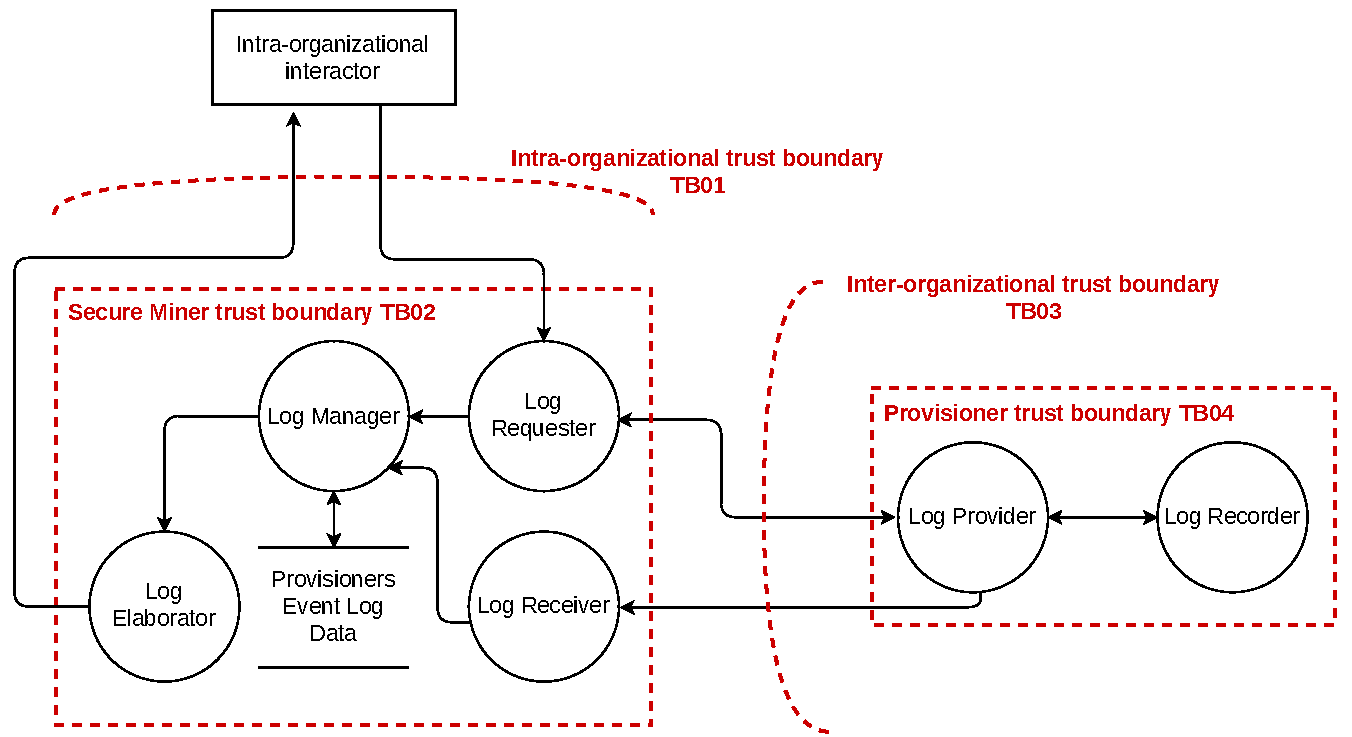
\includegraphics[width=0.95\linewidth]{content//figures/threatmodel.pdf}
    \caption{Data flow diagram employed for our threat model}
    \label{fig:threatmodel:dataflow}
\end{figure}
\begin{table}[t]
\label{table:threatmodel:threats}
\resizebox{\textwidth}{!}{%
    \centering
    \begin{tabular}{llll}\toprule
        \textbf{ID} & \textbf{Trust boundary}& \textbf{Type}  & \textbf{Threat description}\\ \midrule
        T01& \multirow{3}{*}{\makecell[l]{TB01}}& Spoofing   & The attacker impersonates a legitimate interactor to use the \Compo{Secure Miner}\\
        T02&     & Tampering  & The intra-organizational interactor sends malicious input to the \Compo{Secure Miner}\\
        T03&     & Information disclosure  & The attacker sniffs the messages between the interactor and the \Compo{Secure Miner}\\ \midrule
        T04& \multirow{4}{*}{\makecell[l]{TB02}}& Information disclosure  & The attacker accesses the \Compo{Secure Miner}'s memory location to leak the event logs\\ 
        T05& & Tampering  & The attacker meddles the source code of the \Compo{Secure Miner} or its event log data\\
        T06& & Elevation of privileges  & The attacker gains the rights to run in the same environment of the \Compo{Secure Miner}\\
        T07& & Denial of service  & The \Compo{Secure Miner} crashes, halts or stops\\ \midrule
        T08& \multirow{6}{*}{\makecell[l]{TB03}}& Spoofing  & The attacker impersonates a \Compo{Secure Miner} to gain access to the \Compo{Provisioner}'s log\\ 
        T09& & Spoofing  & The attacker impersonates a \Compo{Provisioner} to communicate with the \Compo{Secure Miner}\\
        T010& & Denial of service &The \Compo{Secure Miner} floods the \Compo{Provisioner} with log requests\\
        T010& & Denial of service &The \Compo{Secure Miner} floods the \Compo{Provisioner} with log requests\\
        T011& & Information disclosure & The attacker sniffs the \Compo{Provisioner}'s log sent to the \Compo{Secure Miner}\\ 
        T012& & Tampering & The attacker alters the data flow between the \Compo{Provisioner} and the \Compo{Secure Miner}\\
        \bottomrule
        
        
        
        
    \end{tabular}
    \caption{Vulnerabilities in the CONFINE architecture}
}
\end{table}
\begin{newj}
	

In the following section, we identify the threats that can jeopardize the confidentiality of provisioners' event logs in CONFINE. Our threat analysis is based upon the theoretical foundation of the \textit{STRIDE} framework \cite{aa}. This model groups the threats into six categories: spoofing (i.e., the impersonation of a legitimate entity), tampering (i.e., the modification of data to alter its integrity), repudiation (i.e., the denial of performing a particular action), information disclosure (i.e., the exposure of sensitive data), denial of service (i.e., the disruption or degradation of availability) and elevation of privileges (i.e., the misappropriation of higher level of rights). With the help of the dataflow depicted in \cref{fig:threatmodel:dataflow}, we demarcate the \textit{trust boundaries} (i.e., transitions of trust level) among the CONFINE components. Trust boundary boxes (the red dashed squares in \cref{fig:threatmodel:dataflow}) indicate entities with mutual trust. Therefore, we group the sub-components of the \Compo{Secure Miner} and the \Compo{Provisioner} in the TB02 and TB04 boundary boxes, respectively. The trust boundariesTB01 and TB02 
\todo[inline]{
Introduce \cref{fig:threatmodel:dataflow} adoption;\\
Describe each boundary box with their adversary type (Provisioner --> honest, Secure Miner and input sources--> semi-honest)\\
Explain TB02 AND TB01;\\
For each TBi: describe all the STRICE threats that are in our scope
}

\end{newj}


